\documentclass[border=3mm,tikz,preview]{standalone}
\usepackage[utf8]{inputenc}
\usepackage{amsmath,amssymb,amsfonts}
\usepackage{graphicx}
\usepackage{tikz}
\usetikzlibrary{shapes.geometric, arrows.meta, positioning, shadows, calc, fit, backgrounds}
\usepackage{xcolor}
\begin{document}

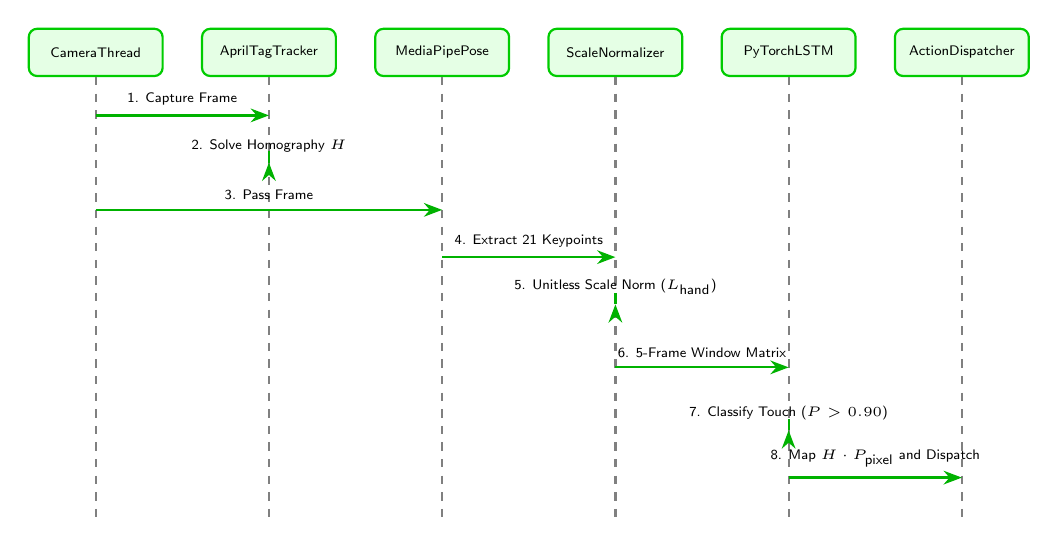
\begin{tikzpicture}[
    lifeline/.style = {draw=black!50, dashed, thick},
    entity/.style = {rectangle, draw=green!80!black, fill=green!10!white, thick, rounded corners=3pt, align=center, font=\sffamily\tiny, minimum width=1.7cm, minimum height=0.6cm},
    msg/.style = {draw=green!70!black, ->, >=Stealth, thick, font=\sffamily\tiny},
    reply/.style = {draw=green!70!black, ->, >=Stealth, dashed, thick, font=\sffamily\tiny}
]

% Entities
\node (cam) [entity] at (0, 0) {CameraThread};
\node (april) [entity] at (2.2, 0) {AprilTagTracker};
\node (mp) [entity] at (4.4, 0) {MediaPipePose};
\node (norm) [entity] at (6.6, 0) {ScaleNormalizer};
\node (lstm) [entity] at (8.8, 0) {PyTorchLSTM};
\node (disp) [entity] at (11.0, 0) {ActionDispatcher};

% Lifelines
\draw [lifeline] (cam) -- (0, -6.0);
\draw [lifeline] (april) -- (2.2, -6.0);
\draw [lifeline] (mp) -- (4.4, -6.0);
\draw [lifeline] (norm) -- (6.6, -6.0);
\draw [lifeline] (lstm) -- (8.8, -6.0);
\draw [lifeline] (disp) -- (11.0, -6.0);

% Messages
\draw [msg] (0, -0.8) -- node[above]{1. Capture Frame} (2.2, -0.8);
\draw [msg] (2.2, -1.4) -- node[above]{2. Solve Homography $H$} (2.2, -1.4);
\draw [msg] (0, -2.0) -- node[above]{3. Pass Frame} (4.4, -2.0);
\draw [msg] (4.4, -2.6) -- node[above]{4. Extract 21 Keypoints} (6.6, -2.6);
\draw [msg] (6.6, -3.2) -- node[above]{5. Unitless Scale Norm ($L_{\text{hand}}$)} (6.6, -3.2);
\draw [msg] (6.6, -4.0) -- node[above]{6. 5-Frame Window Matrix} (8.8, -4.0);
\draw [msg] (8.8, -4.8) -- node[above]{7. Classify Touch ($P > 0.90$)} (8.8, -4.8);
\draw [msg] (8.8, -5.4) -- node[above]{8. Map $H \cdot P_{\text{pixel}}$ and Dispatch} (11.0, -5.4);

\end{tikzpicture}

\end{document}
